\documentclass[11pt]{article}

\def\articlename{资产定价}
\def\authorname{杨弘毅}
\def\startdate{2021年6月10日}

\ifx \authorname\undefined
  \def\authorname{杨弘毅}
\else
\fi

\author{\authorname}
\date{创建:\startdate \\修改:\today}

\usepackage[a4paper,left=6em,right=6em]{geometry}
\usepackage{amsmath,amsfonts,amsthm,bbold}
\usepackage{booktabs,float,multirow}
\usepackage{cancel}
\usepackage{enumitem}
\usepackage{multicol}
\usepackage{graphicx}
\usepackage[toc,title]{appendix}
\usepackage{tikz}
\usetikzlibrary{arrows.meta}
\usetikzlibrary{patterns}
\usetikzlibrary{decorations.pathreplacing}
\usetikzlibrary{decorations.pathmorphing}
\usepackage{subcaption}
\usepackage{fancyhdr}
\pagestyle{fancy}
\setlength{\headheight}{15pt}
\usepackage{footmisc}
\usepackage{hyperref}
\usepackage{tocloft}
\hypersetup{
    colorlinks=true, %set true if you want colored links
    linkcolor=blue,
    linktoc=all, %set to all if you want both sections and subsections linked
    citecolor=black,
    filecolor=black,
    urlcolor=blue
}
\usepackage[UTF8]{ctex}

\title{\articlename}

% Format
\setlength{\cftbeforesecskip}{6pt}
\setlength{\parskip}{0.6em}
\renewcommand{\baselinestretch}{1.4}
\setlist{noitemsep,itemindent=1em,topsep=0em,leftmargin=4em,rightmargin=4em}
\setlist[2]{leftmargin=2em}

% Shortcut
\newcommand{\divider}{\vspace{-\parskip}\noindent\rule{\linewidth}{0.4pt}}
\newcommand{\tops}[1]{\texorpdfstring{#1}{TEXT}}

% Theorem
\newtheorem{thm}{定理}[section] 
\newtheorem{proposition}[thm]{命题}
\newtheorem{lemma}[thm]{引理}
\newtheorem{corollary}[thm]{推论}
\newtheorem{property}[thm]{性质}
\newtheorem{example}[thm]{例子}
\newtheorem{remark}[thm]{备注}
\newtheorem{note}[thm]{注释}

% Symbol
\newcommand{\E}{\mathbb{E}}
\newcommand{\mcl}{\mathcal{L}}
\newcommand{\rnE}{\widetilde{\mathbb{E}}}
\newcommand{\wt}[1]{\widetilde{#1}}
\DeclareMathOperator{\Var}{Var}
\DeclareMathOperator{\Cov}{Cov}
\newcommand{\abs}[1]{\left\lvert #1\right\rvert}
\newcommand{\norm}[1]{\left\lVert #1\right\rVert}
\newcommand{\given}{\:\vert\:}

\begin{document}
\maketitle
\tableofcontents

\section{TODO}
\begin{itemize}
    \item campbell-shiller分解
\end{itemize}

\section{基础}

\subsection{CAPM与APT}

资本资产定价模型(Capital Asset Pricing Model,CAPM)的诞生,才首次清晰的描绘出风险与收益率之间的关系。根据CAPM模型,资产的预期超额收益率由如下一元线性方程决定:
\begin{equation*}
    \E[R_i] - R_f = \beta_i \left( \E[R_M]-R_f \right)
\end{equation*}

其中$R_i$为某资产$i$的收益率,$R_f$为无风险收益率,$\E[R_M]$为市场组合的预期收益率,$\E[R_m]- R_f$为市场风险溢价(Market risk premium),也称为市场因子。其中有$\beta_i = \frac{\Cov(R_i,R_M)}{\Var(R_M)}$,$\beta$刻画了该资产$i$收益对于市场收益的敏感程度,也被称为资产$i$对市场风险的暴露程度。

随后Ross(1976)提出了著名的套利定价理论(Arbitrage Pricing Theory,APT),为多元线性模型:
\begin{equation*}
    \E[R_i^e] = \bm{\beta_{i}^{'} \lambda}
\end{equation*}

同CAPM模型相同,$\bm{\beta}$为因子暴露(Factor exposure)或称为因子载荷(Factor loading),即该目标因子的收益率变化对股票超额收益变化的影响程度(控制其他因子后)。$\bm{\lambda}$是因子预期收益率(Factor expected return),或称为因子溢价(Factor risk premium)或因子风险溢酬。由此可见,资产$i$的预期超额收益率$\E[R_i^e]$,为等式右侧一系列因子的预期收益率,以及该资产在这些因子上的暴露决定。

此时研究的是不同资产之间的预期超额收益率的差别,称为(横)截面(Cross-sectional)差异,而非时间序列(Time-series)或时序上的差异。因子代表了收益率的一种结构,给定了结构与因子预期收益率,不同资产预期超额收益率的差别,由其在这些因子上的暴露决定。\uline{那么多因子模型研究的核心问题,是找到一组能够解释股票预期收益率界面差异的因子}。

\begin{figure}[H]
    \centering
    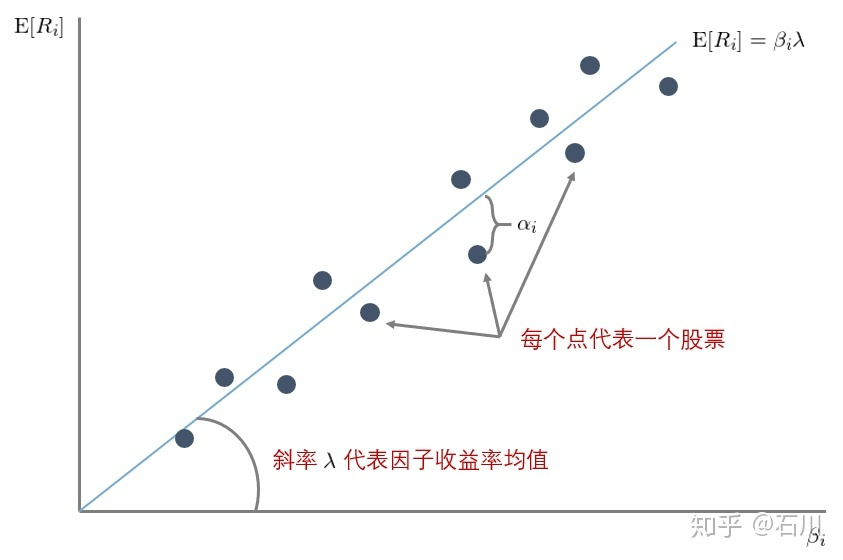
\includegraphics[width=0.6\textwidth]{fig/capm_sml.jpg}
    \caption{CAPM:Security Market Line}
    \label{fig:sml}
\end{figure}

有几点需要注意,在这里使用$\E[\bm{R_i^e}]$为代表资产的预期超额收益率,而非如CAPM中表示的$\E[R_i] - R_f$,是因为在实证中,经常采用多空对冲建立投资组合,此时便无需再减去无风险收益率。另外,学界研究的对象始终为资产的预期草娥收益,因此有时将“超额”二字省略。

\subsection{异象}

而在实际过程中,等式两侧并不相等,而存在着定价误差$\alpha_i$(Pricing error):
\begin{equation*}
    \E[R_i^e] = \alpha_i + \bm{\beta_{i}^{'} \lambda}
\end{equation*}

定价误差有可能由两方面产生:
\begin{itemize}
    \item 模型设定偏误,即等式右侧遗漏了重要的因子,当被遗漏因子加入后,可消除定价误差
    \item 模型设定没有问题,但由于资产收益的实际数据只是总体的一个样本,那么误差总是存在的,此时需要通过统计的方法检验误差$\alpha_i$是否显著不为零:
    \begin{itemize}
        \item 若$\alpha_i$并非显著偏离于零,则出现只是样本问题
        \item 若$\alpha_i$\textbf{显著偏离零},则说明了可以通过套利而获得超额收益的机会,市场对该资产出现错误定价(Mispricing),从而导致了实际预期收益率与多因子模型下的预期收益率出现偏离
    \end{itemize}
\end{itemize}

假使我们根据基本面特征或量价指标等特征,挑选出一揽子股票并构建\uline{多空投资组合}。若该组合的收益率(方程左侧)无法被多因子模型(方程右侧,如3因子、4因子、5因子模型)解释,则称该特征为一个\textbf{异象}(Anomaly)。即该特征获得了多因子模型无法解释$alpha$收益率,但从有效市场假说出发,市场中不应该存在很多异象。同时在学界不断的挖掘中,获得了400+个异象,且在样本内都获得了很高的t-statistics,这里可能存在两个原因:
\begin{itemize}
    \item 数据挖掘,大量的异象在样本内被挖掘出,因此Harvey,Liu和Zhu(2016)提出异象收益率的t-statistic至少要超过3.0,而非传统的5\%显著性对应的2.0,才可能真正有效,而非来源于运气
    \item 模型相关,若以$CAPM$为定价模型,那么许多异象都能获得CAPM无法解释的$\alpha$收益率,同时随着定价模型中因子个数的增加,更多的异象变得不再显著,而真正的定价模型是未知的
\end{itemize}

Hou,Xue和Zhang(2017)长达146页对异象的研究中,复现了学术界提出的 447 个异象,涵盖动量(57个)、价值/成长(68个)、投资(38个)、盈利(79个)、无形资产(103个)、以及交易摩擦(102个)六大类。对于这447个异象,在排除了微小市值股票的影响后,其中286个(64\%),在5\%的显著性水平下不再显著(下同)。若按照Harvey,Liu和Zhu(2016)的建议把t-statistic的阈值提升到3.0,其中380个(85\%)异象不再显著。最后,如果使用Hou,Xue和Zhang(2015)提出的4因子模型作为定价模型,那么其中436个(98\%)异象不再显著,仅有 11个异象显著。

对于超额收益,学术界和业界主流的两种解释是错误定价和风险补偿,错误定价意味着投资者可以通过合理的策略获得潜在的超额收益;而风险补偿则意味着投资者获得的收益是以承担额外风险为代价的。

\subsection{因子}

因子代表了不同资产收益率的某种驱动力,而该因子的收益率就是这些资产的共性收益(同涨同跌)。而如同估值、GDP这些抽象的因子,都可以通过\uline{因子模拟投资组合}(Factor mimicking porfolio)的方式,将抽象概念转换为实际载体,从而进行定量研究。构建因子模拟投资组合需要满足两个条件:
\begin{itemize}
    \item 该投资组合在该目标因子上有大于零的暴露、且在其他因子上的暴露为零(纯粹的反应目标因子收益)
    \item 该投资组合的特质性风险(Idiosyncratic risk),即个股收益率在时序上的随机扰动,在所有满足上述条件的投资组合中最小(减少随机扰动带来的误差)
\end{itemize}

异象有可能能成为优秀的因子,但不是所有异象都是因子。因为作为一个因子(Factor),需要能够解释资产(个股或投资组合)预期收益率截面上的差异,并有增量贡献。具体而言:
\begin{itemize}
    \item 异象从方程的左侧,移动到右侧称为一个因子,称为解释变量,需要考察期是否能解释预期收益率截面上的差异
    \item 由于多个异象之间并不完全独立,需要排除相关性的影响,考察是否有增量贡献
\end{itemize}

如价值因子,也可以采用$E/P$或$B/P$构建High-Minus-Low组合,若同时使用,两者相关性必然很高,因此若使用其一作为价值因子,另一因子对资产预期收益率截面差异的解释能力的增量贡献将变得很低,无法称为因子。

对于因子模型接下去的问题就是,在构建多因子模型时:选取因子因子的数目;以及选取哪些因子。第一个问题,因遵循简约法则(The Law of Parsimony),或奥卡姆剃刀(Occam's razor)。若从ICAPM(Intertemporal CAPM)的角度理解多因子模型,每个因子应代表某种状态变量(State variable),即为投资者想要对冲的某种风险。因此,因子的个数应该是有限的。目前主流的多因子模型如下:
\begin{itemize}
    \item Fama-French 三因子模型(Fama and French 1993):多因子模型的开山鼻祖,包括MKT、HML以及SMB三因子。其中包含了MKT市场因子,HML价值因子,与SMB规模因子
    \item Carhart 四因子模型(Carhart 1997):在 Fama-French三因子模型上加上了动量MOM因子。
    \item Novy-Marx四因子模型(Novy-Marx 2013):包含MKT,HML,MOM以及PMU四个因子,其中 PMU 所用的财务指标是Gross Profit-to-Asset,代表Profitability维度
    \item Fama-French 五因子模型(Fama and French 2015):Fama和French在其三因子模型的基础上加入了CMA和RMW两个因子,分别代表Investment和Profitability 两个维度。
    \item Hou-Xue-Zhang 四因子模型(Hou, Xue and Zhang 2015):包含MKT,SMB,IVA以及ROE。其中IVA是Total assets的年增长率,代表Investment 维度
    \item Stambaugh-Yuan四因子模型(Stambaugh and Yuan 2016):包含MKT,SMB,MGMT和PERF四个因子。MGMT和PERF分别使用了6个和5个指标,代表Management以及 Performance相关的两个Mispricing因子。虽然该模型只有四个因子,但它用到的基本面和量价指标多达 12 个。
    \item Daniel-Hirshleifer-Sun三因子模型(Daniel, Hirshleifer and Sun 2018):在MKT的基础上,使用PEAD和FIN两个指标作为短期和长期行为因子(Behavioral factors)的代理指标,构建了三因子模型。该模型由于包括了传统的MKT市场因子,又包括行为因子,故称为复合模型。
\end{itemize}

对于第二个问题,则涉及了不同多因子模型之间的比较。目前学界主要有三种方法:
\begin{itemize}
    \item GRS tests
    \item Mean-Variance Spanning tests
    \item Bayesian approach
\end{itemize}

【待整理】

GRS tests(Gibbons,Ross和Shanken 1989)检验n个资产在给定因子模型下的定价错误$\alpha$,是否在统计上联合为零(jointly equal to zero)。在比较两个多因子模型时,使用两个模型的因子互为资产和定价模型进行检验。

Mean-Variance Spanning tests考察n个已知资产构建的mean-variance有效前沿能否包含某个新资产(Huberman和Kandel 1987)。在比较两个多因子模型时,使用每个模型的因子构建有效前沿,并逐一检验其能否包含另一个模型中的因子。

在Bayesian approach中,假设比较两个多因子模型$M_1$和$M_2$,数据集使用$D$表示。令 $P(M_1)$和$P(M_2)$为这两个模型的先验概率,且有$P(M_1) + prob(M_2) = 1$(这里假设把多个模型两两比较)。根据贝叶斯定理有:
\begin{equation*}
    P(M_i \given D) = \frac{P(M_i)P(D \given M_i)}{P(M_1)P(D\given M_1) + P(M_2)P(D\given M_2)}
\end{equation*}

其中:
\begin{equation*}
    P(D \given M_i) = \int_{\theta_i} P(\theta_i) P(D \given \theta_i) d\theta_i
\end{equation*}

上式中,$P(\theta_i)$是模型$i$参数的先验分布,$P(D \given \theta_i)$是模型$i$的似然函数。上述贝叶斯方法的核心在于确定$P(\theta_i)$。根据Pastor和Stambaugh(2000) 以及Barillas和Shanken(2018)的理论,它和以两个模型中的全部因子作为资产所构成的投资组合的预期最大夏普率的平方与市场夏普率的比值有关。

\subsection{系统性风险}

【待整理】

除了市场因子以外的风险都是可以被分散的,所以只要是超过市场组合收益的部分都叫做超额收益。

多因子模型的表达式同样强调,只有那些影响众多资产收益率共同运动的风险,而非资产的特质性风险(即可以通过分散化规避掉的风险),才是预期收益率的来源。

系统风险(Systematic risk)的暴露程度,即对于市场风险暴露的大小。即资产的预期超额收益率,由市场组合(市场因子)的预期超额收益率与该资产对市场风险的暴露大小决定。或可以理解为,单项资产的$\beta$系数是指资产预期超额收益率与市场组合预期超额收益率之间变动关系的敏感程度。

系统性风险(Systematic risk),又称市场风险或不可分散风险,是影响所有资产的、不能通过资产组合而消除的风险。这部分风险是由那些影响整个市场的风险所引起的,无论怎样分散投资,也不可能消除系统性风险。避免集中投资于单一市场可减少系统性风险。单项资产、证券资产组合或不同公司受系统性风险影响不一样,系统性风险的大小通常用beta系数($\beta$系数)来衡量。

\section{方法论}

\subsection{排序法}

\subsubsection{因子收益率}

如上所述,构建因子模拟投资组合,即获得因子收益率,需要知道所有股票在该因子上的暴露。即因子暴露是,构建因子模拟投资组合,计算因子收益率的前提。而个股在某因子$k$上的暴露为,在控制其他因子之后,该目标因子$k$的收益率与股票超额收益的敏感程度。即需要已知因子收益率才能计算因子暴露。这样就陷入了“先有鸡还是先有蛋”的困境。

而使用排序法(Portfolio sort)可以避免这样的困境,排序法的核心思想在于使用个股在该变量(因子)上的取值大小,来代替个股在该因子上暴露的高低。需要注意其中并没有假设两者之间满足某种特定的数学关系,仅假设变量与因子暴露是相关联的。即假设高BM取值的股票,在围绕BM构建的价值因子上暴露更高,相反,低BM的股票在围绕BM构建的价值因子上的暴露更低。

如公司财务信息如股票估值、市值、盈利等为最主流的一类因子,称为股票风格因子(Style factor),而围绕GDP的这类经济数据构建的因子这称为宏观经济因子。从此可以看出,排序法仅适用于风格因子,因为对于宏观经济因子,很难从股票自身出发,找到与该变量的联系。可以理解为,风格因子对应了个股自身属性,而宏观经济因子为外在环境,很难再个股自身找到对应。因而不适用与排序法。排序法大致可分为如下三个步骤:
\begin{itemize}
    \item 排序:确定股票池,并将其中全部股票在截面上按照排序变量的高低取值进行排序
    \item 分组:按排名高低将全部股票分为N组,做多排名最高的第一组股票,做空排名最低的最后一组股票,从而构建一个多空对冲组合,或称为价差组合(Spread portfolio)。价差组合的收益率即为变量取值最高的$1/N$支股票的收益率,与变量取值最低的$1/N$支股票收益率之差,即围绕该变量构建的\uline{因子收益率}。还需要注意两点,首先,做多组合,与做空组合应该是资金中性的(Dollar neutral),即两个投资组合的金额相同。其次由于多、空组合都包含多支股票,因此需要对个股进行加权,一般有市值加权与等权重两种方法。
    \item 更新:由于个股在因子上的暴露是随着时间变化的,因此需要定期重复进行上述排序、分组两步,完成对因子模拟投资组合的更新,在学术上也称为再平衡(Rebalance),频率一般为每月或每年。计算当前时刻至下一个再平衡时刻的收益率,如此往复,就可以得到因子收益率的时间序列
\end{itemize}

【思考】如上所述,因子收益率是所有股票共性的收益来源,不同股票在在这些因子收益率上的暴露不同,从而造成了截面上的差别。如果只考虑如BM这样的变量,并不能作为所有共性的部分。在Barra中直接作为暴露?需标准化处理

\subsubsection{检验}

检验因子预期收益率,原假设为因子预期收益率为零,而由定义可知因子的预期收益率应大于零。令$\{\lambda_t\} \; (t=1,2,\dots,T)$代表因子收益率时间序列,因子预期收益率的估计$\hat{\lambda}$以及其标准误分别为:
\begin{gather*}
    \hat{\lambda} = \frac{1}{T}\sum_{t=1}^{T} \lambda_t \\
    s.e.(\hat{\lambda}) = \frac{\sigma(\lambda_t)}{\sqrt{T}}
\end{gather*}

$\{\lambda_t\}$在时序上取平均值,就得到预期因子收益率的估计,这样即可进行t-检验,满足自由度为$T-1$的t分布:
\begin{equation*}
    t\text{-statistic} = \frac{\hat{\lambda}}{s.e.(\hat{\lambda})}
\end{equation*}

\subsubsection{多重排序法}

上述方法使用单一变量对股票排序,称之为单变量排序(Univariate sorting)。根据如上所述因子模拟投资组合的所需满足的条件,应该仅在目标因子上有暴露,在非目标因子上没有暴露。而如上BM的例子中,做多BM最高组,做空BM最低组,其中还包含了对于其他因子的暴露,如市值等,这样就造成估计误差,难以准确估计BM因子。为了排除其他因子的干扰,常见的做法时使用多个变量,进行双重排序(Double sorting或Bivariate sorting)或三重排序(Triple sorting),这些方法统称为多重排序法。

根据排序过程中先后或依存的关系,又可分为独立双重排序(Independent double sorting或Unconditional double sorting),或条件双重排序(Dependent double sorting或Conditional double sorting)。在\uline{独立双重排序}中,假设排序变量为$X_1$与$X_2$,分别独立的将股票划分为$ 2 \times 3$组,一共得到6个投资组合,常见做法是取这两个变量的各自分位数(Quantile)进行分组。如同单变量排序,构建围绕$X_1$的因子收益率,都需做多高$X_1$组合,并做空低$X_1$组合。对于变量$X_2$的每一档内,都有高$X_1$组合,与低高$X_1$组合。那么此时在t期,$X_1$因子的收益率$\lambda_{X_1,t}$为:
\begin{align*}
    \lambda_{X_1,t} &= \frac{1}{3} \left[ R_{(2,1),t} + R_{(2,2),t} + R_{(2,3),t} \right] - \frac{1}{3} \left[R_{(1,1),t} + R_{(1,2),t} + R_{(1,3),t} \right] \\
    &= \frac{1}{3} \left[ R_{(2,1),t} - R_{(1,1),t} \right] + \frac{1}{3} \left[R_{(2,2),t} - R_{(1,2),t} \right] + \frac{1}{3} \left[ R_{(2,3),t} - R_{(1,3),t} \right]
\end{align*}

同理,在t期,$X_2$因子收益率$\lambda_{X_2,t}$为
\begin{align*}
    \lambda_{X_2,t} &= \frac{1}{2} \left[ R_{(1,3),t} + R_{(2,3),t} \right] - \frac{1}{2} \left[R_{(1,1),t} + R_{(2,1),t} \right] \\
    &= \frac{1}{2} \left[ R_{(3,1),t} - R_{(1,1),t} \right] + \frac{1}{2} \left[R_{(3,2),t} + R_{(1,2),t} \right]
\end{align*}

如上所述,多重排序法是为了排除非目标因子的干扰。使用双重排序,学者们也同时考察已有因子的每组内,异象因子是否能解释股票收益率的截面差异。如要检验$X_1$是否能构建异象,还应该考察在$X_2$每组内,根据$X_1$划分的多空组合收益率是否显著。另外独立双重排序可能还存在使得某些组包含股票过少的问题,而使用\uline{条件双重排序}可以解决这个问题。条件双重排序与独立双重排序最大的不同,是按照给定的先后顺序进行排序,如先将$X_1$划分为3组,而后再在$X_1$每组之内,对$X_2$进行划分,最终得到$3\times 2$组,这样保证了每组内有足够的股票。

条件双重排序,核心为考察控制了$X_1$之后,变量$X_2$对股票收益率的影响。此时两个变量的重要性与排序的先后顺序有关,由于第一排序变量仅为控制变量,而第二排序变量与收益率之间的关系更为重要。因此也只需围绕第二排序变量,构建因子模拟投资组合,并计算因子收益率,方法与计算独立双重排序时相同

\subsection{多因子模型}

假设N与K代表资产和因子的个数,对于多因子截面关系式:
\begin{equation*}
    \E[R_{i}^{e}] = \alpha_i + \bm{\beta_{i}^{'} \lambda}
\end{equation*}

在上述截面关系式中,$R_{i}^{e}$为资产i的超额收益率(或直接记作$R_{i}$),$\bm{\beta}_i$为资产i在K个因子上的因子暴露向量,$\bm{\lambda}$为K个因子的收益率向量。\uline{多因子模型研究的核心问题是资产预期收益率在截面之间为什么有差异}。由上式可见,其并不关心时序上的波动,只关心超额收益率的期望$\E[R_{i}^{e}]$与$\bm{\beta}_i$之间截面上的关系(收益与风险)。因子代表了收益率的一种结构(线性关关系),结构一旦确定,资产的收益率就由因子暴露决定,暴露高,收益率就高。

目标是找到一种好的因子结构,使得个股在截面上的预期收益率区分度高,并且使得模型不能解释的定价误差$\alpha_i$尽可能小。若能够在统计上证明所有股票的$\alpha_i$都接近零,这说明这样的因子结构能够较好的解释个股截面预期收益率的差别。因此,多因子模型的回归检验中的重中之重,就是所有$\alpha_i$联合起来是否在统计上足够接近零。

因此,多因子模型的回归检验可以总结为:
\begin{itemize}
    \item 选择因子,并计算每个资产在这些因子上的暴露$\bm{\beta}_i$
    \item 找到个股超额收益率均值$\E[R_{i}]$和因子暴露$\beta_i$在截面上的关系,即进行回归分析
    \item 计算个股的定价误差$\alpha_i$,联合检验这些$\alpha_i$是否在统计上为零
    \item 检验每个因子的预期收益率$\lambda_k$
\end{itemize}

注意:超额收益率为t+1期,而因子为t期,即Lead-lag回归。下文所有向量都为列向量,其转置为行向量。
\begin{equation*}
    \bm{a} = \begin{bmatrix}
        a_1 \\
        a_2 \\
        \vdots \\
        a_n
    \end{bmatrix}
    \qquad
    \bm{a}' = \begin{bmatrix}
        a_1 & a_2 & \dots a_n \\
    \end{bmatrix}
\end{equation*}

\subsection{时序回归}

时间序列回归(Time-series regression)最为简单直接,Black等(1972)最早使用其来检验CAPM。使用因子收益率作为自变量,以资产的超额收益率作为因变量。如上文所述的风格因子,使用排序法构建的因子模拟投资组合,其收益率如经典的HML,SMB等,那么此时可以通过时序回归,来分析个股超额收益率$\E[R_i]$与因子暴露$\beta_i$之间在截面上的关系。由于宏观经济因子难以使用排序法构建因子模拟投资组合并计算其收益率,难以使用时序回归。

对于资产i,进行时间序列回归,即:
\begin{equation*}
    R_{i,t}^{e} = \alpha_i + \bm{\beta}_{i}^{'} \bm{\lambda}_t + \varepsilon_{i,t} \inlinesep t=1,2,\dots,T
\end{equation*}

当有N个资产和K个因子时,在$\bm{\lambda}$前加入单列常数1为截距,矩阵形式有:
\begin{equation*}
    \underset{T \times N}{\bm{R}} = \underset{ T \times (K+1)}{\bm{\lambda}} \underset{(K+1) \times N}{\hat{\bm{\beta}}} + \underset{T \times N}{\bm{\epsilon}}
\end{equation*}

其中:
\begin{gather*}
    \bm{R} = \begin{bmatrix} \bm{R}_1 & \dots & \bm{R}_N \\ \end{bmatrix}
    = \begin{bmatrix} R_{1,1} & \dots & R_{1,N} \\ \vdots & \vdots & \ddots \\ R_{T,1} & \dots & R_{T,N} \end{bmatrix} \\
    \bm{\lambda} = \begin{bmatrix} \bm{\lambda}_{1}^{'} \\ \vdots \\ \bm{\lambda}_{T}^{'} \end{bmatrix}
    = \begin{bmatrix} 1 & \lambda_{1,1} & \dots & \lambda_{1,K} \\ \vdots & \vdots & \ddots & \vdots \\ 1 & \lambda_{T,1} & \dots & \lambda_{T,K} \end{bmatrix} 
    \\
    \hat{\bm{\beta}}
    = \begin{bmatrix} \bm{\hat{\beta}}_{0}^{'} \\ \bm{\hat{\beta}}_{1}^{'} \\ \vdots \\ \bm{\hat{\beta}}_{K}^{'} \end{bmatrix}
    = \begin{bmatrix} \hat{\beta}_{0,1} & \dots & \hat{\beta}_{0,N} \\ \hat{\beta}_{1,1} & \dots & \hat{\beta}_{1,N} \\ \vdots & \ddots & \vdots \\ \hat{\beta}_{K,1} & \dots & \hat{\beta}_{K,N} \end{bmatrix}
    \\
    \bm{\epsilon} = \begin{bmatrix}
        \bm{\epsilon}_1 & \dots & \bm{\epsilon}_N \\
    \end{bmatrix}
    = \begin{bmatrix} \epsilon_{1,1} & \dots & \epsilon_{1,N} \\ \vdots & \vdots & \ddots \\ \epsilon_{T,1} & \dots & \epsilon_{T,N} \end{bmatrix}
\end{gather*}

注意在\verb|Python|中,\verb|statsmodel.OLS|对于多因变量回归(Y为多列)一并回归,与对单因变量(Y为单列)逐列回归结果相同。其中$\bm{\beta}_{0}^{'}$为截距,即为$\bm{\alpha}^{'}$,或可以写为:
\begin{gather*}
    \hat{\bm{\beta}}
    = \begin{bmatrix} \bm{\alpha}^{'} \\ \bm{\beta}_{1}^{'} \\ \vdots \\ \bm{\beta}_{K}^{'} \end{bmatrix}
    = \begin{bmatrix} \alpha_{1} & \dots & \alpha_{N} \\ \beta_{1,1} & \dots & \beta_{1,N} \\ \vdots & \ddots & \vdots \\ \beta_{K,1} & \dots & \beta_{K,N} \end{bmatrix}
\end{gather*}

这样就获得了全部资产$i=1,\dots,N$在因子上的暴露向量$\hat{\bm{\beta}}_i$,截距$\hat{\alpha}_i$以及残差$\hat{\bm{\epsilon}}_i$。由于对资产i在时序上进行回归,那么对$R_{t,i}$与$\lambda_t$在时序上取均值,得到$\E_T[R_{t,i}]$和$\E_T[\bm{\lambda_t}]$。因此对于每个资产i,都有如下关系:
\begin{equation*}
    \E_T[R_i] = \alpha_i + \bm{\beta_{i}^{'}} \E_T[\bm{\lambda_t}] \inlinesep i=1,2,\dots,N
\end{equation*}

事实上,当自变量为因子收益率时,仅靠对个资产进行时序回归,就可以获得所有资产在截面上的关系。为方便理解,假设单因子情形进行作图,图中红线为$\E_T[R_i] = \beta_i \E_T[\lambda_t]$,那么对于N个资产,每个资产i都对应图上$(\beta_i,\E[R_i])$一点,此时斜率为因子收益率$\hat{\lambda}=\E_T[\lambda_t]$。将当$\beta_i=0$时,即暴露为0,与$\beta_i=1$代入,暴露为1,为因子投资组合。可知该直线过$(0,0)$与$(1,\hat{\lambda})$两点。而时序回归得到的截距$\alpha_i$即为资产i的定价误差,即为此时各个资产到该直线的距离。Black,Jensen和Scholes(1972) 基于如上的论述给出了时序回归法中求解因子预期收益率的简单方法,因子收益率$\bm{\lambda}_t$,在时序上的均值就是因子的预期收益率$\hat{\bm{\lambda}} = \E_T[\bm{\lambda_t}]$。

\begin{figure}[H]
    \centering
    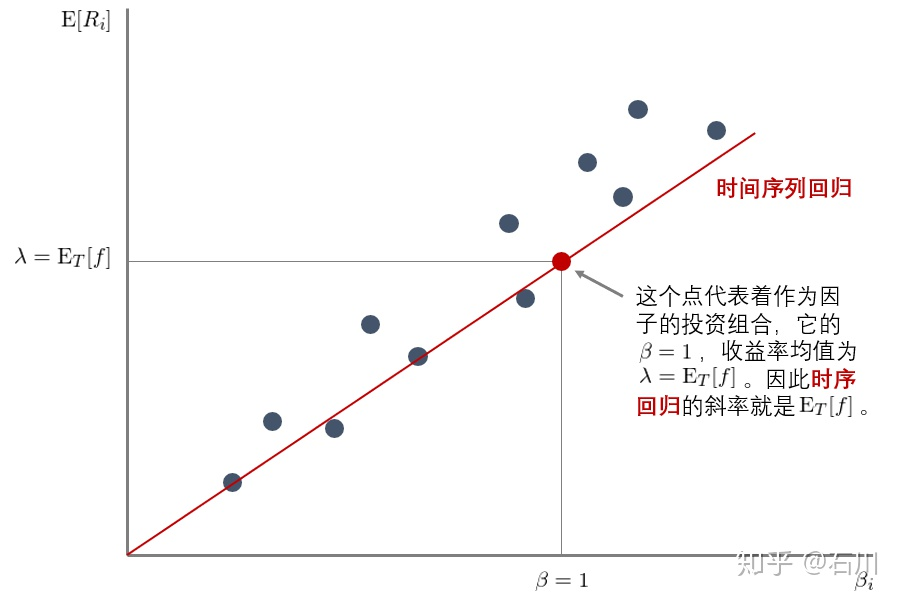
\includegraphics[width=0.8\textwidth]{fig/ts_reg.jpg}
    \caption{时序回归}
    \label{fig:ts_reg}
\end{figure}

这样就通过了时序回归,得到了个股超额收益率与因子暴露在截面上的关系。注意,此时的截面关系并非通过OLS得到,因此直线并不是最小化定价误差$\alpha_i$的平方和为目标求出的。由于是在时序上进行OLS回归,因此其最小化资产i,在时序上的误差$\epsilon_{t,i}$的平方和。

对于检验$\alpha_i$联合起来是否统计上为零,若残差不相关和同方差,标准误可以由OLS标准公式计算。若残差满足独立同分布且为正态分布,可以使用GRS检验,由Gibbons
,Ross和Shanken(1989)提出。而当残差之间存在相关性或者异方差,则需要使用GMM才能得到准确的估计以及标准误,GMM由Lars Peter Hansen于1982年提出。

\subsection{截面回归}

时序回归虽然方便,但仅限于处理股票风格类因子,因子收益率为已知。相比于时序回归,截面回归的优势是,因子的选择范围更广,可以为GDP、CPI、利率等宏观经济指标,可以处理因子收益率时间序列收益率未知的情形。

\subsubsection{方法}

与时序回归相同,第一步仍然需要确定因子暴露$\bm{\beta}$,假设在t时刻,K因子的取值为:
\begin{equation*}
    \bm{F}_t =
    \begin{bmatrix}
        F_{1,K} \\
        F_{2,K} \\
        \vdots \\
        F_{t,K} 
    \end{bmatrix}
\end{equation*}

那么此时,对于资产i,进行时序回归应有:
\begin{equation*}
    R_{i,t} = a_i + \bm{\hat{\beta}}_{i}^{'} \bm{F}_t + \varepsilon_{i,t} \inlinesep t=1,2,\dots,T
\end{equation*}

由于此时的解释变量$\bm{F_t}$并非因子收益率,因此截距$a_i$并非定价误差。当有N个资产和K个因子时,在$\bm{\lambda}$前加入单列常数1为截距,矩阵形式有:
\begin{equation*}
    \underset{T \times N}{\bm{R}} = \underset{ T \times (K+1)}{\bm{F}} \underset{(K+1) \times N}{\hat{\bm{\beta}}} + \underset{T \times N}{\bm{\epsilon}}
\end{equation*}

其中:
\begin{gather*}
    \bm{R} = \begin{bmatrix} \bm{R}_1 & \dots & \bm{R}_N \\ \end{bmatrix}
    = \begin{bmatrix} R_{1,1} & \dots & R_{1,N} \\ \vdots & \vdots & \ddots \\ R_{T,1} & \dots & R_{T,N} \end{bmatrix} \\
    \bm{F} = \begin{bmatrix} 1 & \bm{F}_{1}^{'} \\ \vdots & \vdots \\ 1 & \bm{F}_{T}^{'} \end{bmatrix}
    = \begin{bmatrix} 1 & F_{1,1} & \dots & F_{1,K} \\ \vdots & \vdots & \ddots & \vdots \\ 1 & F_{T,1} & \dots & F_{T,K} \end{bmatrix} 
    \\
    \hat{\bm{\beta}}
    = \begin{bmatrix} \bm{\hat{a}}^{'} \\ \bm{\hat{\beta}}_{1}^{'} \\ \vdots \\ \bm{\hat{\beta}}_{K}^{'} \end{bmatrix}
    = \begin{bmatrix} \hat{a}_{1} & \dots & \hat{a}_{N} \\ \hat{\beta}_{1,1} & \dots & \hat{\beta}_{1,N} \\ \vdots & \ddots & \vdots \\ \hat{\beta}_{K,1} & \dots & \hat{\beta}_{K,N} \end{bmatrix}
    \\
    \bm{\epsilon} = \begin{bmatrix}
        \bm{\epsilon}_1 & \dots & \bm{\epsilon}_N \\
    \end{bmatrix}
    = \begin{bmatrix} \epsilon_{1,1} & \dots & \epsilon_{1,N} \\ \vdots & \vdots & \ddots \\ \epsilon_{T,1} & \dots & \epsilon_{T,N} \end{bmatrix}
\end{gather*}

得到了个股因子暴露$\beta$之后,就可以进行第二步截面回归。此时等式左边为$\E_T[R_i]$为整个T其的收益率均值,而右侧为时序回归得到的$\bm{\beta_i}$。对于N个资产,每个资产i都对应点$(\bm{\beta_i},\E[R_i])$。此时对所有资产,进行截面回归:
\begin{equation*}
    \E[R_i] = \bm{\hat{\beta}}_{i}^{'} \bm{\lambda} + \alpha_i \inlinesep \forall i=1,2,\dots,N
\end{equation*}

矩阵形式应有:
\begin{equation*}
    \underset{N \times 1}{\bm{R}} = \underset{N \times K}{\hat{\bm{\beta}}^{'}} \underset{ K \times 1}{\bm{\lambda}} + \underset{N \times 1}{\bm{\alpha}}
\end{equation*}

其中:
\begin{gather*}
    \bm{R} = \begin{bmatrix} \E_T[R_1] \\ \vdots \\ \E_T[R_N] \end{bmatrix}
    \qquad
    \hat{\bm{\beta}}^{'}
    = \begin{bmatrix} \bm{\hat{\beta}}_{1}^{'} \\ \vdots \\ \bm{\hat{\beta}}_{N}^{'} \end{bmatrix}
    = \begin{bmatrix} \hat{\beta}_{1,1} & \dots & \hat{\beta}_{1,K} \\ \vdots & \ddots & \vdots \\ \hat{\beta}_{N,1} & \dots & \hat{\beta}_{N,K} \end{bmatrix}
    \\
    \bm{\lambda} = \begin{bmatrix} \lambda_{1} \\ \vdots \\ \lambda_{K} \end{bmatrix}
    \qquad
    \bm{\alpha} = \begin{bmatrix} \alpha_1 \\ \dots \\ \alpha_N \end{bmatrix}
\end{gather*}

注意,此时截面回归的残差为定价误差$\alpha_i$,但由于只进行了一次回归,因此只能得到\uline{单组}定价误差$\bm{\alpha}$与\uline{单组}因子预期收益率$\bm{\lambda}$。并且在进行截面回归时没有加入截距项的原因为,多因子模型假设不存在模型设定偏误,资产的预期收益率应仅由因子暴露和因子预期收益率决定。但又如Cochrane(2005)中所指出,也可以考虑包含截距项$\bm{\gamma}_t$的回归模型:
\begin{equation*}
    \E_T[R_{i}] = \bm{\gamma}_i + \hat{\bm{\beta}}_{i}^{'} \bm{\lambda} + \alpha_{i} \inlinesep \forall i=1,2,\dots,N
\end{equation*}

\begin{figure}[H]
    \centering
    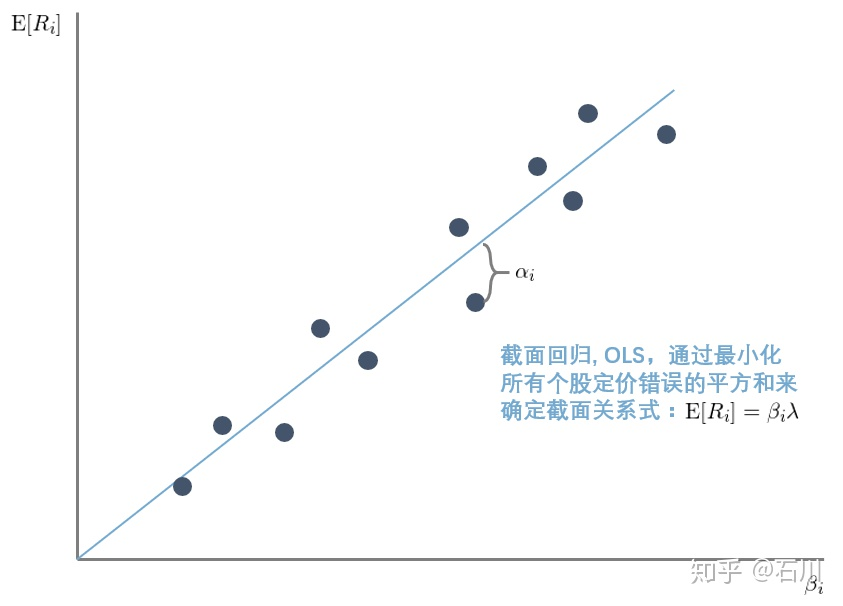
\includegraphics[width=0.8\textwidth]{fig/cs_reg.jpg}
    \caption{传统截面回归}
    \label{fig:cs_reg}
\end{figure}

因此截面回归,也称为两步回归估计(Two-pass regression estimate)。首先,通过时序回归首先得到个股对因子的暴露。其次,对超额收益率取均值,即个股转换为点$(\beta_i,\E[R_i])$,并对N支个股同时进行截面回归,最终得到定价误差与因子收益率,因此截面回归通过最小化所有资产定价误差$\alpha_i$平方和的方式来确定截面关系。

\subsubsection{检验}

【待整理】

对于因子收益率与定价误差,估计量有:
\begin{align*}
    \hat{\bm{\lambda}} &= \left( \bm{\hat{\beta}^{'} \hat{\beta}}\right)^{-1} \bm{\hat{\beta}}^{'} \bm{R} \\
    \hat{\bm{\alpha}} &= \bm{R} - \bm{\hat{\beta} \hat{\lambda}}
\end{align*}

为了联合检验,还需要知道各自的标准误

由于截面个股残差的相关性,虽然不会影响OLS估计,但会导致OLS给出的标准误存在较大误差,因此可以使用GLS取代OLS,由于GLS考虑了残差的协方差因此可以得到准确的标准误。但估计残差的协方差矩阵在现实中有较大的障碍。此时则可使用GMM,由于截面回归的$\bm{\hat{\beta}}_i$并非使用因子收益率回归得到,而是通过时序回归出的估计值(Generated regressors),存在误差。Shanken(1992)给出了修正方法(Shanken correction)。同时利用Shanken correction与GMM,即可检验$\alpha_i$是否联合为0。

\subsection{时序回归 vs 截面回归}

对于时序回归而言,通过对因子收益率在时序取均值$\bm{\lambda} = \E_T[\bm{\lambda}_t]$,来得到隐含的截面关系。因此$\E[R_i] = \bm{\beta}_{i}^{'} \bm{\lambda}$必然过原点$(0,0)$,以及因子收益率的投资组合$(1,\bm{\lambda})$($\bm{\beta_i}=1$)。而在截面回归中,因子暴露已经通过时序回归确定,而在第二次进行截面回归时,充分使用了个股数据。若使用OLS进行截面回归,以最小化个股定价误差$\alpha_i$的平方和为目标。因子收益率通过回归得到,与时序中直接通过计算均值的方式不同,更加合理。

\begin{figure}[H]
    \centering
    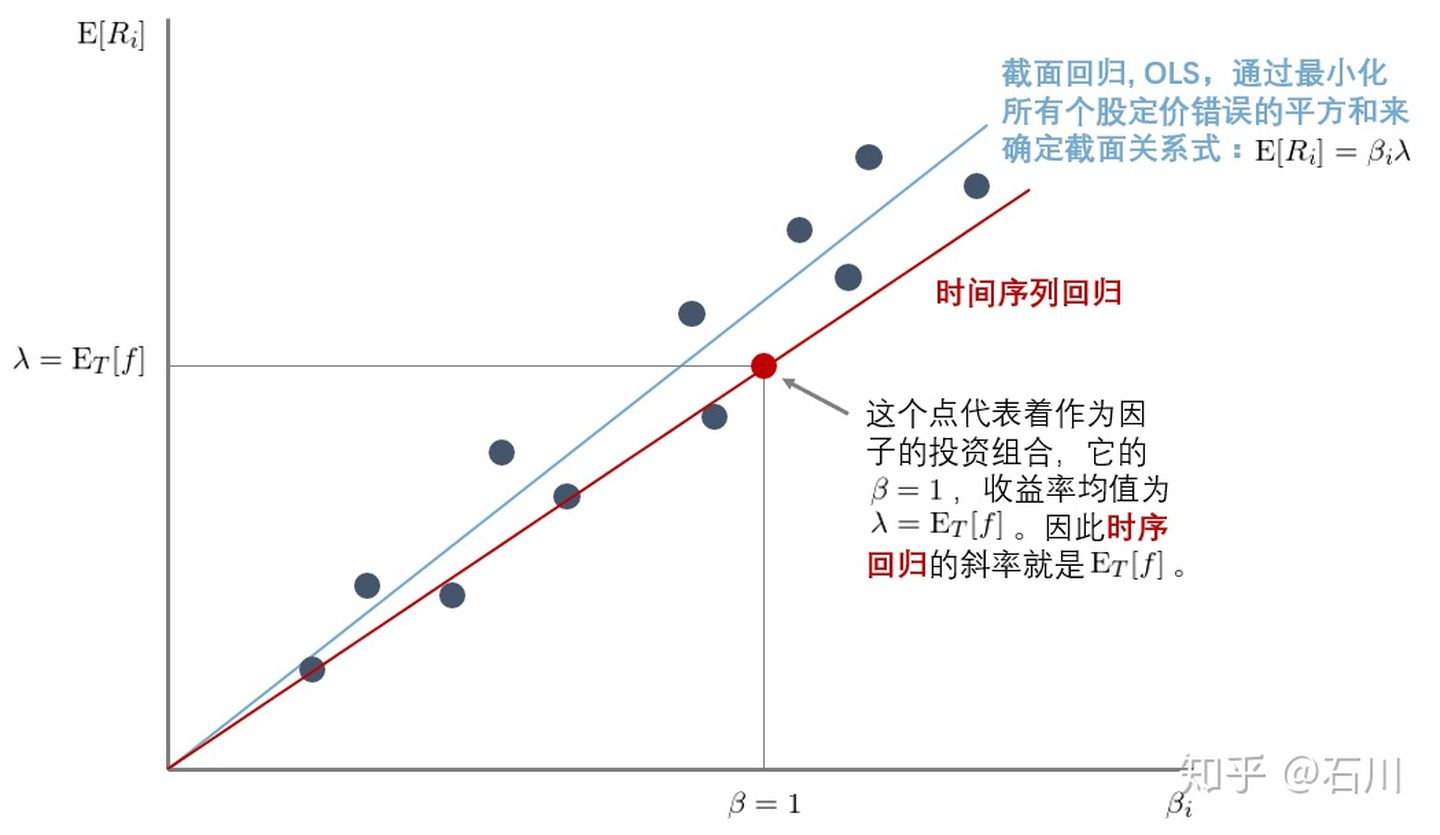
\includegraphics[width=0.8\textwidth]{fig/ts_vs_cs.jpg}
    \caption{时序回归与截面回归}
    \label{fig:ts_vs_cs}
\end{figure}

\subsection{Fama-MacBeth回归}

\subsubsection{方法}

在Fama和MacBeth(1973)中,提出了Fama-MacBeth截面回归,目的是为了检验 CAPM。Fama-MacBeth截面回归也分为两步,但与传统截面回归有所不同。首先,与传统截面回归相同,也需要先进行时序回归,得到资产i超额收益率$R_i$在因子上的暴露$\bm{\beta}_i$。在第一步中,又可分为因子暴露$\bm{\beta}_i$不变与$\bm{\beta}_i$时变两种情形。对于因子暴露不变的情形,对$t=1,\dots,T$整体时序样本,只进行一次时序回归,得到一个不随时间改变的因子暴露。由于$\bm{\beta_i}$不变,那么对于传统截面回归的先均值再回归,与FM截面回归的先回归再均值,两种方式在所有T期上得到的估计是相同的(但FM截面回归在检验上一定的优势)。

在Fama和MacBeth(1973)中,采用滚动窗口的方法估计$\bm{\beta_i}$,因此对于不同的t,$\bm{\beta_i}$随时间改变。
\begin{equation*}
    \bm{R}_{i,t} = \bm{a}_i + \bm{\beta_{i} \bm{F}_t + \bm{\varepsilon}_{i,t}} \inlinesep \forall t=1,2,\dots,T
\end{equation*}

其次,在传统截面回归中,如上节所述,第二步只进行一次截面回归。即对资产i的超额收益率$\bm{R}_i = \begin{bmatrix} R_{1,i} \\ \vdots \\ R_{T,i} \end{bmatrix}$在时序上取均值得到$\E_T[\bm{R}_i]$,与该资产i的因子暴露$\bm{\beta}_i$进行回归,只进行了\uline{1次回归}:
\begin{equation*}
    \E_T[\bm{R}_i] = \bm{\beta_{i}^{'} \lambda_i} + \bm{\alpha}_i \inlinesep \forall i=1,2,\dots,N
\end{equation*}

而在Fama-MacBeth截面回归中,第二步并不对$R_{i,t}$在时序上取均值,需要对在$t=1,\dots,T$期上各进行一次截面回归,一共进行\uline{T次回归},得到T组因子收益率$\bm{\lambda}_t$与T组定价误差$\bm{\alpha}_t$:
\begin{equation*}
    \bm{R}_{i,t} = \bm{\beta}_{i}^{'} \bm{\lambda}_{i,t} + \bm{\alpha}_{i,t} \inlinesep \forall i=1,2,\dots,N
\end{equation*}

因子暴露$\hat{\bm{\beta}}$由上一步得到(可为不变或时变)为估计值,以不变为例,对于第t期而言,写为矩阵形式为:
\begin{equation*}
    \underset{N \times 1}{\bm{R}_t} = \underset{N \times K}{\hat{\bm{\beta}}^{'}} \underset{ K \times 1}{\bm{\lambda}_t}  + \underset{N \times 1}{\bm{\alpha}_t}
\end{equation*}

其中:
\begin{gather*}
    \bm{R}_t = \begin{bmatrix}R_{1,t} \\ \vdots \\ R_{N,t}\end{bmatrix}
    \qquad 
    \hat{\bm{\beta}}^{'} = 
    \begin{bmatrix} \bm{\hat{\beta}}_{1}^{'} \\ \vdots \\ \bm{\hat{\beta}}_{N}^{'} \end{bmatrix} =
    \begin{bmatrix} \hat{\beta}_{1,1} & \dots & \hat{\beta}_{1,K} \\ \vdots & \ddots & \vdots \\ \hat{\beta}_{N,1} & \dots & \hat{\beta}_{N,K} \end{bmatrix}
    \\
    \bm{\lambda}_t = \begin{bmatrix}\lambda_{1,t} \\ \vdots \\ \lambda_{K,t} \end{bmatrix}
    \qquad
    \bm{\alpha}_t = \begin{bmatrix}\alpha_{1,t} \\ \vdots \\ \alpha_{N,t} \end{bmatrix}
\end{gather*}

进行T次回归后,可以得到K个因子随时间变化的因子收益率$\bm{\lambda}$,与N个资产随时间变化的定价误差$\bm{\alpha}$:
\begin{gather*}
    \underset{K \times T}{\bm{\lambda}} = \begin{bmatrix} \bm{\lambda}_{1}^{'} \\ \vdots \\ \bm{\lambda}_{K}^{'} \end{bmatrix} = 
    \begin{bmatrix} \lambda_{1,1} & \dots & \lambda_{1,T} \\ \vdots & \ddots & \vdots \\ \lambda_{K,1} & \dots & \lambda_{K,T} \end{bmatrix}
    \qquad
    \underset{N \times T}{\bm{\alpha}} = \begin{bmatrix} \bm{\alpha}_{1}^{'} \\ \vdots \\ \bm{\alpha}_{N}^{'} \end{bmatrix} =
    \begin{bmatrix} \alpha_{1,1} & \dots & \alpha_{1,T} \\ \vdots & \ddots & \vdots \\ \alpha_{N,1} & \dots & \alpha_{N,T} \end{bmatrix}
\end{gather*}

Fama-MacBeth截面回归和传统截面回归的相同点和区别是:
\begin{itemize}
    \item FM回归与截面回归,都需先进行时序回归,以确定个股的因子暴露$\bm{\beta_i}$
    \item 传统截面回归将$R_{i,t}$在时序上取均值得到$\E[R_i]$,再进行1次截面回归,得到$\alpha_i$和$\lambda$
    \item 对于FM回归,在各个不同的t时刻使用$R_{i,t}$与$\bm{\beta_{i}}$进行回归,再将回归结果在时序上取均值得到$\alpha_i = \E[\alpha_{i,t}]$与$\lambda=\E[\lambda_t]$
    \item 即传统回归为先取均值,后回归。而FM回归为先回归,后取均值
\end{itemize}

注意,如上所述,若使用滚动方法,即$\bm{\beta}$时变。在实际回归过程中,采用Lead-lag回归的方法,即对于$t$期,使用截止$t-1$期的一段给定窗口的历史数据进行第一步的时序回归,估计$\hat{\bm{\beta}}_{i,t-1}$。并且使用其作为第二步$t$期截面回归的解释变量,得到因子收益率:
\begin{equation*}
    \bm{R}_{i,t}^{e} = \hat{\bm{\beta}}_{i,t-1} \bm{\lambda}_t + \bm{\alpha}_{i,t} \inlinesep \forall i=1,2,\dots,N
\end{equation*}

或如Cochrane(2005)中,在截面回归中加入截距项$\bm{\gamma}_t$:
\begin{equation*}
    \bm{R}_{i,t}^{e} = \bm{\gamma}_t + \hat{\bm{\beta}}_{i,t-1} \bm{\lambda}_t + \bm{\alpha}_{i,t} \inlinesep \forall i=1,2,\dots,N
\end{equation*}

\subsubsection{检验}

那么此时对于$\alpha_{i,t}$与$\lambda_t$都有T次回归结果。对于单个资产i,从$t=1$时刻到$t=T$时刻,有$\left(\bm{\beta_{i,1}},\E[R_{i,1}]\right),\left(\bm{\beta_{i,2}},\E[R_{i,2}]\right),\dots,\left(\bm{\beta_{i,T}},\E[R_{i,T}]\right)$。即可以以此估计定价误差以及因子收益率:
\begin{align*}
    \hat{\lambda} &= \frac{1}{T} \sum_{t=1}^{T} \lambda_t \\
    \hat{\alpha}_i &= \frac{1}{T} \sum_{t=1}^{T} \alpha_{i,t}
\end{align*}

不同于传统截面回归,只得到$\lambda$和$\alpha$的一个样本估计,在FM截面回归中得到T个$\lambda$和$\alpha$的样本估计,这样就可以求出两者标准误为:
\begin{align*}
    \sigma^2(\hat{\lambda}) &= \frac{1}{T^2} \sum_{t=1}^{T} \left( \hat{\lambda}_t - \hat{\lambda} \right)^2 \\
    \sigma^2(\hat{\alpha}_i) &= \frac{1}{T^2} \sum_{t=1}^{T} \left( \hat{\alpha}_{i,t} - \hat{\alpha}_i \right)^2
\end{align*}

【待整理】

Fama-MacBeth 也是一个两步截面回归检验方法;它非常巧妙排除了残差在截面上的相关性对标准误的影响,

由上面的介绍可知,Fama-MacBeth 回归的最大优点是它排除了残差截面相关性对标准误的影响。股票的残差收益率在截面上具有很高的相关性,因此该修正对于准确计算标准误至关重要。下面来说说它的不足。首先,Fama-MacBeth 回归对于残差在时序上的相关性无能为力。如果残差在时序上存在相关性,则需要对 Fama-MacBeth 回归得到的标准误进一步修正。Petersen (2009) 分析了不同的回归技术在分析面板数据(panel data)时由于忽略残差的时序或截面相关性而导致不准确的标准误(低估了其真实值)。这篇文章非常值得一读。其次,上文提到,在截面回归中用到的$\bm{\beta}_i$并不是已知的,而是通过时间序列得到的估计值(generated regressors),因此存在误差。Fama-MacBeth 回归对此也无能为力,需要 Shanken correction。

\subsection{Barra多因子模型}

Barra多因子模型也是截面回归模型,其考虑了行业因子和来自基本面和技术面的风格因子。但与传统的截面回归模型不同的是在Barra模型中,因子暴露并非来自时间序列回归,而是直接来自基本面或者技术面数据本身。

例如Book-to-Market ratio,在Fama-French三因子模型中,其被用来构建HML(High-Minus-Low)投资组合,投资组合的收益率作为因子。由时序回归决定个股在这个因子上的暴露,与个股实际的BM无关。但在Barra模型中,BM直接用于确定因子暴露,但需要进行标准化。有了因子暴露,Barra截面模型与传统截面模型相同,都是通过截面回归确定因子收益率。因此,Barra 模型(业界代表)和学术界流行的因子模型最大的不同就是因子暴露$\bm{\beta_i}$的确定。

对于两种确定因子暴露的方法,通过时间序列得到的$\bm{\beta}$,经过平滑,变化更加缓慢。而直接使用基本面数据获得$\bm{\beta}$,可以更快的捕捉公司的变化。需要注意的是,这些因子都需要进行标准化,不能直接使用原始数据。例如,公司市值不经过标准化而作为因子暴露,公司市值差异巨大。假设A公司市值为B公司的100倍,此时显然不能说A公司的超额收益率对于市值因子的暴露为B公司的100倍。所以对于市值因子或其他\uline{风格因子},常见的是首先取对数,然后再进行标准化。对于其他的风格因子,也需要采用相应的标准化处理。在Barra的文档中对如何标准化因子暴露有详细的说明。对于行业因子,Barra将因子暴露处理为Binary变量或虚拟变量,例如工商银行在银行业的暴露为1,而在其他行业的暴露为0。

\subsection{GRS}

\subsection{GMM}

GMM,它可以轻松的求出我们需要的各种量(Hansen 功不可没啊)。另外值得一提的是,在截面回归时用到的$\beta_i$并不是已知、真实的,而是从时间序列回归得出的估计值,它们称为 generated regressors,存在误差。Shanken (1992) 给出了解决该问题的修正方法,称为 Shanken correction。利用 Shanken correction 和 GMM,就可以检验$\alpha$是否为零了。

如今我们有了 GMM 这样的大杀器,能够方便的处理残差的各种相关性。

\appendix

\begin{appendices}

\section{APT推导}

第一步,假设资产的收益率,在单因子情形下,满足如下线性模型:
\begin{equation*}
    R_i = \mu_i + \beta_i f + \varepsilon_i \inlinesep i =1,\dots,n
\end{equation*}

此时$R_i$为资产收益率,$\mu_i$资产$i$的预期收益率,$\beta_i$是资产在因子上的暴露,而$f$是因子取值,而非因子风险溢酬,$\varepsilon_i$为资产$i$收益率的随机扰动或特质性收益率,并满足$\E[f]=\E[\varepsilon_i]=0$,若改写为向量形式,为Ross在APT中使用的收益率模型,有:
\begin{equation*}
    \bm{R} = \bm{\mu + f\beta + \varepsilon}
\end{equation*}

第二步,构建一个arbitrage portfolio,这个投资组合中资产的权重$\omega$满足如下两点特性。首先,该投资组合是零额投资的,即:
\begin{equation*}
    \bm{w' 1 = 0}
\end{equation*}

其中有$\bm{1}$为全为1的向量。其次,并且$\bm{w'\beta}=0$,即该投资组合在该因子上的暴露为零。此时这个投资组合的收益率应为:
\begin{equation*}
    R_p = \bm{w'R = w'\mu + w'\beta f + w'\varepsilon}
\end{equation*}

由上可知,这个投资组合的收益率可化简为:
\begin{equation*}
    R_p = \bm{w'R = w'\mu} 
\end{equation*}

第三步,运用无套利约束,可知根据$\bm{w}$构建的投资组合有如下性质:零额投资;对因子的暴露为零(因此该组合没有系统性风险);没有特质性风险暴露(因为组合中特质性收益率为零)。换言之,这样一个投资组合,既没有资金投入又没有风险暴露,因此根据无套利约束条件,它的收益率必须为零,即:
\begin{equation*}
    R_p = \bm{w'\mu} = 0
\end{equation*}

根据几何可知,$w' 1 = w' \beta = w'\mu = 0$,说明$\bm{w'}$与$\bm{1}$,$\bm{\beta}$和$\bm{\mu}$,都相互垂直。因此$\bm{\mu}$必然在$\bm{1}$和$\bm{\beta}$构成的平面内。

\begin{figure}[H]
    \centering
    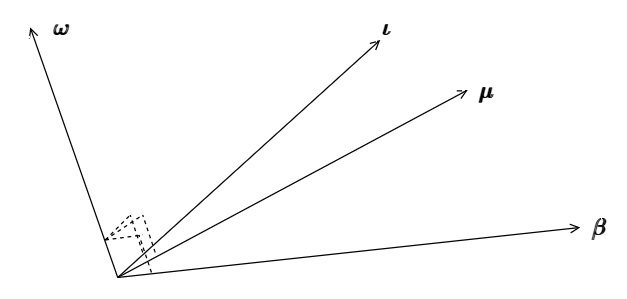
\includegraphics[width=0.6\textwidth]{fig/apt.jpg}
    \caption{APT}
    \label{fig:apt}
\end{figure}

因此在数学上,资产预期收益率$\bm{\mu}$可以写成$\bm{1}$与$\bm{\beta}$的线性组合,即:
\begin{equation*}
    \bm{\mu} = \gamma_1 \bm{1} + \gamma_2 \bm{\beta}
\end{equation*}

那么此时上式应对任何资产都成立,为了求解$\gamma_1$与$\gamma_2$可代入特殊资产,无风险资产($R_f$),与市场组合($R_M$)。由于无风险资产的因子暴露为零,代入上式可得:
\begin{equation*}
    R_f = \gamma_1
\end{equation*}

对于市场组合,其$beta=1$,并将$\gamma_1 = R_f$代入,可得:
\begin{equation*}
    R_M = R_f + \gamma_2 \times \bm{1}
\end{equation*}

因此有:
\begin{equation*}
    \gamma = R_M - R_f
\end{equation*}

代入原式,最终可得到CAPM的表达式:
\begin{equation*}
    \mu_i = R_f + \beta_i(R_M - R_f)
\end{equation*}

在此基础上,扩展至多因子,即得到APT模型:
\begin{equation*}
    \E[R_{i}^{e}] = \mu_i - R_f = \beta_{i,1} \lambda_1 + \beta_{i,2} \lambda_2 + \dots + \beta_{i,K} \lambda_K
\end{equation*}

\end{appendices}

\end{document}